\chapter{EXPERIMENTAL RESULTS AND PERFORMANCE ANALYSIS}
\label{chap:ch4}





\section{DATASET DESCRIPTION}\label{sec:ch4_1}

\subsection{Source Datasets and Versions}\label{sec:ch4_1_1}

The project pools three public 12-lead ECG cohorts, each identified by the exact release obtained (Section 3.3.1). Table~\ref{tab:ch4_1} gives, for each cohort, the release, the source of its diagnostic labels and the number of recordings at each stage of preparation. The counts are those written by the preprocessing stage (\url{data/processed_100hz/preprocessing_summary.json} and the per-cohort summaries) and confirmed by a recount of the Module 4 split manifest (\url{runs/module4_v3/split_manifest.csv}).

{
\setlength{\tabcolsep}{2pt}
\renewcommand{\arraystretch}{1.12}
\begin{table}[htbp]
\centering
\scriptsize
\setstretch{1.0}
\caption{Source Datasets Used in the Project}\label{tab:ch4_1}
\begin{tabular}{|p{0.12\textwidth}|p{0.20\textwidth}|p{0.20\textwidth}|p{0.13\textwidth}|p{0.16\textwidth}|p{0.12\textwidth}|}
\hline
\textbf{Cohort} & \textbf{Release used} & \textbf{Source of diagnostic labels} & \textbf{Recordings processed} & \textbf{Rejected by quality screening} & \textbf{Eligible recordings} \\ \hline
PTB-XL & PhysioNet release 1.0.3 \cite{WAGNER2022PTBXLDATA}; dataset described in \cite{WAGNER2020PTBXL} & SCP-ECG statements assigned by cardiologists \cite{WAGNER2020PTBXL} & 21,799 & 2 & 21,797 \\ \hline
Chapman-Shaoxing & Training set of the PhysioNet/Computing in Cardiology Challenge 2021, release 1.0.3, \url{chapman_shaoxing} subset \cite{CINC2021DATA}; original database \cite{ZHENG2020CHAPMAN} & SNOMED CT codes in the record headers & 10,158 & 16 & 10,142 \\ \hline
MIMIC-IV-ECG & Release 1.0 \cite{GOW2023MIMICIVECG}; subset of 5,000 recordings, one per patient, sampled with seed 42 & Machine-generated interpretation statements distributed with the dataset & 5,000 & 51 & 4,949 \\ \hline
\textbf{Total} &  &  & \textbf{36,957} & \textbf{69} & \textbf{36,888} \\ \hline
\end{tabular}
\end{table}
}

The counts in Table~\ref{tab:ch4_1} describe the project's working subset, which differs from the full releases in two ways. For Chapman-Shaoxing, the records manifest (\url{data/external_validation/chapman/records_manifest.csv}) lists 10,247 recordings, of which 89 had missing files, leaving the 10,158 processed recordings. For MIMIC-IV-ECG, the project's sampling audit (\url{reports/dataset_sampling_audit.json}) records a pool of 800,035 recordings from 161,352 patients, from which the 5,000-recording subset was drawn. PTB-XL release 1.0.3 contains 21,799 recordings, all of which were processed.

The three cohorts were labelled in different ways, and this affects how their results can be compared. PTB-XL labels come from cardiologists. Chapman-Shaoxing labels are diagnosis codes supplied with the Challenge 2021 distribution. MIMIC-IV-ECG labels are derived from the statements of an automated interpretation program, so they show what that program reported, not a clinician's diagnosis. Differences in labelling practice and population between ECG databases are a known source of difficulty for multi-database classification \cite{REYNA2022ISSUES}. The per-cohort results of Section~\ref{sec:ch4_4_5} have to be read with this in mind.

\subsection{Data Partitions}\label{sec:ch4_1_2}

The recordings were divided into training, validation and test partitions by the patient-grouped, label-stratified procedure of Section 3.3.4. Table~\ref{tab:ch4_2} gives the number of recordings and patients in each partition, recounted from the Module 4 split manifest.

\begin{table}[htbp]
\centering
\small
\renewcommand{\arraystretch}{1.12}
\setstretch{1.0}
\setlength{\tabcolsep}{2pt}
\caption{Recordings and Patients in Each Partition}\label{tab:ch4_2}
\begin{tabular}{|p{0.25\textwidth}|p{0.18\textwidth}|p{0.18\textwidth}|p{0.18\textwidth}|p{0.14\textwidth}|}
\hline
\textbf{Cohort} & \textbf{Training (folds 1–7)} & \textbf{Validation (fold 8)} & \textbf{Test (folds 9–10)} & \textbf{Total} \\ \hline
PTB-XL recordings & 15,260 & 2,179 & 4,358 & 21,797 \\ \hline
PTB-XL patients & 13,253 & 1,885 & 3,729 & 18,867 \\ \hline
Chapman-Shaoxing recordings (each treated as one patient) & 7,100 & 1,014 & 2,028 & 10,142 \\ \hline
MIMIC-IV-ECG recordings (one per patient) & 3,465 & 495 & 989 & 4,949 \\ \hline
\textbf{All recordings} & \textbf{25,825} & \textbf{3,688} & \textbf{7,375} & \textbf{36,888} \\ \hline
\textbf{All patients} & \textbf{23,818} & \textbf{3,394} & \textbf{6,746} & \textbf{33,958} \\ \hline
Recording–configuration examples (× 7 configurations) & 180,775 per epoch & 25,816 & 51,625 & 258,216 \\ \hline
\end{tabular}
\end{table}

Each recording is presented in all seven lead configurations, so the 51,625 test examples are seven views of 7,375 recordings from 6,746 patients. They are not 51,625 independent patients, and all test sample sizes in this chapter should be read in that light.

No patient identifier appears in more than one partition, but this check only has force where identifiers exist. PTB-XL and MIMIC-IV-ECG provide patient identifiers. Chapman-Shaoxing does not, so each of its recordings is treated as a separate patient and patient-level separation cannot be established for this cohort. The Module 1 freeze record lists 13 pairs of identical Chapman-Shaoxing signals stored under different record identifiers. The labels of each pair agree. Nine of the pairs cross partitions: six link the training and test partitions, two the training and validation partitions, and one the validation and test partitions. Seven test recordings therefore have exact copies in data used for training or model selection. This is about 0.1\% of the 7,375 test recordings, too few to change the reported metrics in any material way, but it is a genuine leakage and is disclosed as such.

\subsection{Label Distribution}\label{sec:ch4_1_3}

Labels have three states: positive, negative and unknown (Section 3.3.2). Unknown labels are excluded from training and evaluation, so each condition is evaluated on its own subset of recordings. Table~\ref{tab:ch4_3} gives the number of positive labels and the number of known labels for each condition in each partition. The test counts come from the confusion matrices in the saved test summary (\url{runs/module4_v3/metrics/test_evaluation_summary.json}), because test labels are blanked in the split manifest as a quarantine measure.

\begin{table}[htbp]
\centering
\small
\setlength{\tabcolsep}{2pt}
\renewcommand{\arraystretch}{1.12}
\setstretch{1.0}
\caption{Positive Labels / Known Labels (Prevalence) in Each Partition}\label{tab:ch4_3}
\begin{tabular}{|p{0.15\textwidth}|p{0.26\textwidth}|p{0.26\textwidth}|p{0.26\textwidth}|}
\hline
\textbf{Condition} & \textbf{Training} & \textbf{Validation} & \textbf{Test} \\ \hline
NORM & 7,889 / 25,730 (30.7\%) & 1,128 / 3,675 (30.7\%) & 2,225 / 7,347 (30.3\%) \\ \hline
AFIB & 2,716 / 25,212 (10.8\%) & 389 / 3,610 (10.8\%) & 788 / 7,188 (11.0\%) \\ \hline
RBBB & 1,177 / 24,094 (4.9\%) & 167 / 3,416 (4.9\%) & 336 / 6,870 (4.9\%) \\ \hline
LBBB & 963 / 24,797 (3.9\%) & 135 / 3,536 (3.8\%) & 274 / 7,089 (3.9\%) \\ \hline
SBRAD & 3,701 / 21,982 (16.8\%) & 528 / 3,132 (16.9\%) & 1,056 / 6,240 (16.9\%) \\ \hline
STACH & 2,156 / 21,980 (9.8\%) & 304 / 3,133 (9.7\%) & 622 / 6,237 (10.0\%) \\ \hline
1AVB & 995 / 22,414 (4.4\%) & 141 / 3,201 (4.4\%) & 286 / 6,368 (4.5\%) \\ \hline
MI & 4,097 / 22,712 (18.0\%) & 584 / 3,255 (17.9\%) & 1,196 / 6,517 (18.4\%) \\ \hline
\end{tabular}
\end{table}

The stratified split keeps the prevalence of every condition almost identical across the three partitions. The conditions are strongly imbalanced, from about 4\% for left bundle branch block and first-degree atrioventricular block to about 30\% for the normal ECG. The test partition still contains at least 274 positive recordings for every condition, so no per-condition test estimate rests on a very small number of positives. The number of known labels differs by condition, from 6,237 to 7,347 test recordings, and per-condition results are therefore computed over different denominators.

\section{ECOSYSTEM (HARDWARE \& SOFTWARE SPECIFICATIONS)}\label{sec:ch4_2}

The repository has no environment file, package list or saved training log. The specifications in Table~\ref{tab:ch4_4} are therefore limited to what can be established from scripts, run reports and checkpoints. Where a specification is not recorded, the table says so rather than inferring it.

\clearpage
{\small
\setlength{\tabcolsep}{2pt}
\renewcommand{\arraystretch}{1.1}
\setstretch{1.0}
\renewcommand{\UrlFont}{\footnotesize\ttfamily}
\setlength{\LTcapwidth}{\textwidth}
\begin{longtable}{|>{\raggedright\arraybackslash}p{0.18\textwidth}|>{\raggedright\arraybackslash}p{0.47\textwidth}|>{\raggedright\arraybackslash}p{0.28\textwidth}|}
\caption{Hardware, Software and Training Specifications}\label{tab:ch4_4}\\
\hline
\textbf{Item} & \textbf{Specification} & \textbf{Evidence} \\ \hline
\endfirsthead
\multicolumn{3}{c}{\tablename~\thetable{} - continued from previous page} \\ \hline

\endhead
\hline
\multicolumn{3}{r}{} \\
\endfoot
\hline
\endlastfoot
Processor and accelerator used for training & Not recorded in the available experiment artefacts. The Stage 6 report states that 16-thread CPU execution was enabled for Module 4; the training script enables this setting only when it runs on the CPU & \url{runs/module4_v3/reports/stage6_validation_and_audit_report.md}; \url{scripts/16_train_reasoning_transformer.py} \\ \hline
Foundation-model feature extraction & CPU; the extraction script fixes the device to the CPU, and the logs record batch size 32 with 8 threads per worker & \url{runs/module3_v1/scripts/extract_foundation_representations.py}; \url{runs/module3_v1/logs/} \\ \hline
Inference for validation traces & CPU, 16-thread worker pool & \url{runs/module4_v3/reports/validation_trace_generation_report.md} \\ \hline
Memory (RAM, accelerator memory) & Not recorded in the available experiment artefacts & — \\ \hline
Operating system & Windows (test session platform \url{win32}) & Stage 6 report, test-suite output \\ \hline
Python & 3.11.4; pytest 9.1.1 & Stage 6 report, test-suite output \\ \hline
Library versions used for the runs & Not recorded in the available experiment artefacts. The Python 3.11.4 installation on the project machine had PyTorch 2.14.0 (CPU build) when this report was written, but this is not evidence of the version used for the runs & Checked on 19 October 2026 \\ \hline
Foundation model & ECG-FM \cite{MCKEEN2025ECGFM}, \url{wav2vec2_cmsc}, 12 encoder layers, width 768; 90,883,072 parameters, all frozen; checkpoint \url{checkpoints/ecg_fm/mimic_iv_ecg_physionet_pretrained.pt} (SHA-256 beginning \url{4d0142bc}) & \url{configs/control_path_training_config.json}; Module 4 freeze record \\ \hline
Control Reasoning Transformer & 1,830,657 trainable parameters & \url{configs/control_path_training_config.json}; checkpoints \\ \hline
Loss & Binary cross-entropy over known labels (Section 3.3.8) & \url{scripts/16_train_reasoning_transformer.py} \\ \hline
Optimiser & AdamW; learning rate $10^{-4}$; weight decay $10^{-4}$; betas (0.9, 0.999) & Checkpoint optimiser state \\ \hline
Batch size & 64 & Checkpoint step count; script default; Stage 6 report \\ \hline
Learning-rate schedule & Cosine annealing over 15 epochs to $10^{-6}$, no warm-up & Learning-rate history in \url{control_training_history_seed*.json} \\

\end{longtable}
}

The training settings in Table~\ref{tab:ch4_4} are those that the run actually used. The training configuration file specifies a batch size of 32, at most 20 epochs and two warm-up epochs, but the training script uses its own defaults of 64, 15 and none. The saved run confirms this: the seed-42 optimiser state shows 2,825 steps per epoch, which is 180,775 examples in batches of 64, and the recorded learning rates follow a 15-epoch cosine schedule from $10^{-4}$ to $10^{-6}$ without warm-up.


\section{EXPERIMENTS CONDUCTED}\label{sec:ch4_3}

\subsection{Overview of the Experiments}\label{sec:ch4_3_1}

Table~\ref{tab:ch4_5} lists the experiments that were carried out, with the artefact that holds each result, its completion status and its main caveat. An experiment is listed as completed only when its saved output was inspected; the existence of a script was not taken as evidence that it ran.

\clearpage
{\small
\setlength{\tabcolsep}{2pt}
\renewcommand{\arraystretch}{1.0}
\setstretch{1.0}
\renewcommand{\UrlFont}{\footnotesize\ttfamily}
\setlength{\LTcapwidth}{\textwidth}
\begin{longtable}{|>{\raggedright\arraybackslash}p{0.08\textwidth}|>{\raggedright\arraybackslash}p{0.20\textwidth}|>{\raggedright\arraybackslash}p{0.24\textwidth}|>{\raggedright\arraybackslash}p{0.18\textwidth}|>{\raggedright\arraybackslash}p{0.21\textwidth}|}
\caption{Experiments Conducted}\label{tab:ch4_5}\\
\hline
\textbf{No.} & \textbf{Experiment} & \textbf{Evidence artefact} & \textbf{Status} & \textbf{Key caveat} \\ \hline
\endfirsthead
\multicolumn{5}{c}{\tablename~\thetable{} - continued from previous page} \\ \hline
\textbf{No.} & \textbf{Experiment} & \textbf{Evidence artefact} & \textbf{Status} & \textbf{Key caveat} \\ \hline
\endhead
\hline
\multicolumn{5}{r}{Continued on next page} \\
\endfoot
\hline
\endlastfoot
E1 & Dataset preparation and quality screening & \url{data/processed_100hz/*/preprocessing_summary.json}; split manifest & Completed: 36,888 of 36,957 recordings retained & Chapman-Shaoxing has no patient identifiers; 13 duplicate pairs \\ \hline
E2 & Progressive lead masking and representation extraction & \url{runs/module3_v1/} (freeze record, logs, drift reports) & Completed: 258,216 representations, no failures recorded & Input conditions differ from ECG-FM pretraining (Section 3.3.6) \\ \hline
E3 & Clinical observation extraction & \url{runs/module4_v3/observations/} & Completed for all partitions and configurations & QRS measurement ceiling; rhythm-label mismatch (Section~\ref{sec:ch4_4_8}) \\ \hline
E4 & Observation-extractor validation study & \url{reports/clinical_observation_validation.json} & Completed: 250 MIMIC-IV-ECG recordings & Reference values are machine measurements, not clinician readings \\ \hline
E5 & Control Reasoning Transformer training & \url{runs/module4_v3/metrics/control_training_history_seed*.json}; checkpoints & Completed for seeds 42, 1337 and 2024 & Settings differ from the configuration file (Section~\ref{sec:ch4_2}) \\ \hline
E6 & Calibration & Training histories & Completed on the validation partition & Fitted and measured on the same validation data \\ \hline
E7 & Validation evaluation by configuration & Training histories & Completed for all three seeds & Uncalibrated probabilities \\ \hline
E8 & Test evaluation of the Control Reasoning Transformer (B-3) & \url{runs/module4_v3/metrics/test_evaluation_summary.json}; \url{test_predictions_seed42.csv} & Completed for seed 42 only & Authorisation-unverified (Section~\ref{sec:ch4_3_2}) \\ \hline
E9 & Comparison models on the test partition & \url{runs/module4_v3/metrics/comprehensive_baseline_comparison.json} & Completed after E8 & Script outside the repository; no per-recording predictions; B-2 defective \\ \hline
E10 & Representation drift & \url{runs/module3_v1/reports/module3_cosine_similarity_summary.csv} & Completed for all partitions & Measures geometry, not diagnostic accuracy \\ 
\end{longtable}
}

The following parts of the research programme were not carried out in the first half and have no results in this chapter:

\begin{itemize}
\item \textbf{Grounding gate and evidence states (Module 5).} Specified in the internal protocol and evidence schema, not implemented. Section 3.3.9 lists the schema revisions required before implementation.
\item \textbf{Grounding metrics (EO, GQ, TGR, UR, GSR) and the Reasoning Failure Boundary (Module 6).} Not computed, because they need the gate's evidence states.
\item \textbf{Diagnostic Failure Boundary and AURDC.} Not implemented in the evaluation scripts. Section~\ref{sec:ch4_4_3} explains why no DFB is read off the classification results.
\item \textbf{Clinical Knowledge Prior and the knowledge-augmented comparison (B-4).} Planned future work.
\item \textbf{Test evaluation of seeds 1337 and 2024, patient-clustered and paired confidence intervals, and ablations of the observation and lead-availability tokens.} Not run.
\end{itemize}

\subsection{Evaluation Provenance}\label{sec:ch4_3_2}

The protocol requires the test partition to be evaluated once, after an explicit authorisation by the investigator. The project's provenance statement (\url{runs/module4_v3/reports/evaluation_provenance_statement.md}) records that this condition was not met: the evaluation was started by an automated hook of the development environment, the first run stopped because of a software error, and the run was repeated after the error had been fixed. Two further facts bear on the run. The data loader (\url{src/reasoning/multi_cohort_loader.py}) was last modified at 16:08 UTC on 15 October 2026, after the freeze record was written at 06:54 UTC and before the test summary was written at 16:29 UTC, so the evaluation did not use the frozen version of the loader. The test-trace script (\url{scripts/17_generate_reasoning_traces.py}), which also computes the test metrics, is not listed in the freeze record.

The comparison-model results of experiment E9 were produced 23 minutes after the test summary, by a script (\texttt{evaluate\_baselines.py}) stored outside the repository.

For these reasons, every test result in this chapter is a descriptive result from the recorded run. It is not a confirmatory, pre-specified or independently validated evaluation, and the evidence does not establish that the test partition was untouched before the run. The project's post-evaluation audit (\url{runs/module4_v3/reports/post_evaluation_baseline_reconciliation_audit.md}) recomputed the test metrics from the saved predictions and found that they agree with the saved summary to within rounding. Its Stage 7 Markdown report does not fully agree with the summary: it gives 754 instead of 788 positive atrial fibrillation recordings, lists the wrong leads for the 10-lead configuration, and some of its single-lead per-cohort values differ from the summary. Where the two disagree, this chapter uses the saved summary.

\subsection{Evaluation Measures}\label{sec:ch4_3_3}

The measures are those of Section 3.3.11: per-condition AUROC and F1 at a threshold of 0.5 on calibrated probabilities over recordings with a known label, their unweighted macro-averages, and the Brier score, negative log-likelihood (NLL) and expected calibration error (ECE) with 10 equal-width bins \cite{GUO2017CALIBRATION}. The 95\% intervals come from 200 record-level bootstrap resamples, not the 1,000 patient-clustered resamples that the protocol specifies for grounding metrics, so they may be somewhat narrow.

Two distinctions are necessary when results from different partitions are compared. The test metrics are computed from calibrated probabilities. The per-configuration validation metrics saved during training are computed from uncalibrated probabilities, because the training script evaluates each configuration with the model's raw probabilities, without applying the fitted temperatures. And test results exist for seed 42 only, while validation results exist for all three seeds. The pooled three-seed summary saved by the project (\url{runs/module4_v3/metrics/multi_seed_variance_summary.json}) gives a macro-AUROC of 0.9449 ± 0.0006 and a macro-F1 of 0.6982 ± 0.0026. These are validation values pooled over all seven configurations, not test values, and they are not set beside the test results as three-seed test performance.

\section{PERFORMANCE ANALYSIS}\label{sec:ch4_4}

\subsection{Validation Performance and Seed Variability}\label{sec:ch4_4_1}

Table~\ref{tab:ch4_6} gives the validation macro-AUROC and macro-F1 of each seed in each configuration, from uncalibrated probabilities. The spread is the difference between the highest and lowest of the three seeds.

{\scriptsize
\setlength{\tabcolsep}{2pt}
\renewcommand{\arraystretch}{1.12}
\setstretch{1.0}
\setlength{\LTcapwidth}{\textwidth}
\begin{longtable}{|p{0.14\textwidth}|p{0.28\textwidth}|p{0.10\textwidth}|p{0.28\textwidth}|p{0.10\textwidth}|}
\caption[Validation Performance by Seed]{Validation Performance by Seed (Fold 8, 3,688 Recordings per Configuration, Uncalibrated)}\label{tab:ch4_6}\\
\hline
\textbf{Configuration} & \textbf{Macro-AUROC: 42 / 1337 / 2024} & \textbf{Spread} & \textbf{Macro-F1: 42 / 1337 / 2024} & \textbf{Spread} \\ \hline
\endfirsthead
\multicolumn{5}{c}{\tablename~\thetable{} - continued from previous page} \\ \hline
\textbf{Configuration} & \textbf{Macro-AUROC: 42 / 1337 / 2024} & \textbf{Spread} & \textbf{Macro-F1: 42 / 1337 / 2024} & \textbf{Spread} \\ \hline
\endhead
\hline
\multicolumn{5}{r}{Continued on next page} \\
\endfoot
\hline
\endlastfoot
12-lead & 0.9521 / 0.9521 / 0.9499 & 0.0022 & 0.7241 / 0.7272 / 0.7310 & 0.0069 \\ \hline
10-lead & 0.9513 / 0.9513 / 0.9490 & 0.0023 & 0.7191 / 0.7294 / 0.7286 & 0.0103 \\ \hline
8-lead & 0.9500 / 0.9513 / 0.9481 & 0.0032 & 0.7105 / 0.7240 / 0.7218 & 0.0135 \\ \hline
6-lead & 0.9453 / 0.9452 / 0.9447 & 0.0006 & 0.6950 / 0.7022 / 0.6953 & 0.0072 \\ \hline
4-lead & 0.9493 / 0.9492 / 0.9496 & 0.0004 & 0.7158 / 0.7207 / 0.7311 & 0.0153 \\ \hline
2-lead & 0.9451 / 0.9454 / 0.9442 & 0.0012 & 0.6994 / 0.6936 / 0.7043 & 0.0107 \\ \hline
1-lead & 0.9120 / 0.9122 / 0.9111 & 0.0011 & 0.5713 / 0.5498 / 0.5592 & 0.0215 \\ \hline
\end{longtable}
}

{\small Source: \path{runs/module4_v3/metrics/control_training_history_seed*.json} (seeds 42, 1337 and 2024).}

The three seeds produce very similar models. All three reached their lowest validation loss at epoch 3 and stopped at epoch 8, and their best validation losses were 0.15925, 0.15669 and 0.15950. The macro-AUROC of the three seeds differs by at most 0.0032 in any configuration. The macro-F1 varies more, by up to 0.0215 in the single-lead configuration, because a fixed threshold turns small shifts in probability into changes in the number of predicted positives. Because only the seed-42 model was evaluated on the test partition, this seed variability is known for validation only. It suggests that differences between configurations much smaller than about 0.003 in macro-AUROC or 0.02 in macro-F1 should not be interpreted, even before sampling uncertainty is considered.

\subsection{Calibration}\label{sec:ch4_4_2}

The temperatures were fitted per condition on the pooled validation partition (25,816 recording--configuration examples). The fitted temperatures lie between 0.93 and 1.26, with a mean of 1.15 for seed 42, 1.13 for seed 1337 and 1.10 for seed 2024. Most are slightly above 1, which means that the model was slightly overconfident and that calibration softened its probabilities. On the pooled validation partition, temperature scaling reduced the mean ECE from 0.01498 to 0.01043 for seed 42, from 0.01193 to 0.00764 for seed 1337 and from 0.01373 to 0.01180 for seed 2024, a reduction of between 14\% and 36\%. The NLL and Brier score changed only slightly; for seed 42 they fell from 0.15769 to 0.15586 and from 0.04741 to 0.04713 (source: calibration field of the training histories). These validation figures are optimistic, because the temperatures were fitted on the same data on which they are measured. The test partition gives an out-of-sample check: with the seed-42 temperatures, the test ECE ranges from 0.0105 in the 12-lead configuration to 0.0132 in the single-lead configuration (Table~\ref{tab:ch4_7}). This shows that one set of temperatures, fitted on all configurations together, remains usable when leads are removed, with a small rise in calibration error. The test values before calibration were not saved, so the effect of calibration on the test partition cannot be shown.

\subsection{Test Performance Across Lead Configurations}\label{sec:ch4_4_3}

Table~\ref{tab:ch4_7} and Figure~\ref{fig:ch4_1} give the test results of the seed-42 Control Reasoning Transformer in each configuration.

{\scriptsize
\setlength{\tabcolsep}{2pt}
\renewcommand{\arraystretch}{1.12}
\setstretch{1.0}
\setlength{\LTcapwidth}{\textwidth}
\begin{longtable}{|p{0.12\textwidth}|p{0.19\textwidth}|p{0.16\textwidth}|p{0.16\textwidth}|p{0.10\textwidth}|p{0.10\textwidth}|p{0.10\textwidth}|}
\caption[Test Performance by Configuration]{Test Performance of the Control Reasoning Transformer by Configuration (Seed 42, Calibrated, Descriptive)}\label{tab:ch4_7}\\
\hline
\textbf{Configuration} & \textbf{Active leads} & \textbf{Macro-AUROC [95\% CI]} & \textbf{Macro-F1 [95\% CI]} & \textbf{Brier} & \textbf{NLL} & \textbf{ECE} \\ \hline
\endfirsthead
\multicolumn{7}{c}{\tablename~\thetable{} - continued from previous page} \\ \hline
\textbf{Configuration} & \textbf{Active leads} & \textbf{Macro-AUROC [95\% CI]} & \textbf{Macro-F1 [95\% CI]} & \textbf{Brier} & \textbf{NLL} & \textbf{ECE} \\ \hline
\endhead
\hline
\multicolumn{7}{r}{Continued on next page} \\
\endfoot
\hline
\endlastfoot
12-lead & I, II, III, aVR, aVL, aVF, V1–V6 & 0.9540 [0.9514, 0.9572] & 0.7375 [0.7295, 0.7478] & 0.04309 & 0.14367 & 0.01047 \\ \hline
10-lead & I, II, aVR, aVL, V1–V6 & 0.9536 [0.9509, 0.9566] & 0.7367 [0.7278, 0.7483] & 0.04330 & 0.14418 & 0.01071 \\ \hline
8-lead & I, II, V1–V6 & 0.9526 [0.9502, 0.9558] & 0.7307 [0.7228, 0.7421] & 0.04381 & 0.14591 & 0.01100 \\ \hline
6-lead & I, II, III, aVR, aVL, aVF & 0.9479 [0.9450, 0.9510] & 0.7076 [0.6987, 0.7209] & 0.04612 & 0.15259 & 0.01219 \\ \hline
4-lead & I, II, III, V1 & 0.9524 [0.9499, 0.9553] & 0.7347 [0.7253, 0.7461] & 0.04408 & 0.14637 & 0.01247 \\ \hline
2-lead & II, V1 & 0.9487 [0.9455, 0.9519] & 0.7101 [0.7000, 0.7218] & 0.04666 & 0.15322 & 0.01247 \\ \hline
1-lead & II & 0.9215 [0.9175, 0.9251] & 0.5832 [0.5710, 0.5983] & 0.05397 & 0.17846 & 0.01319 \\ \hline
\end{longtable}
}

{\small Source: \path{runs/module4_v3/metrics/test_evaluation_summary.json}; 7,375 test recordings per configuration; intervals from 200 record-level bootstrap resamples.}

\begin{figure}[htbp]
\centering
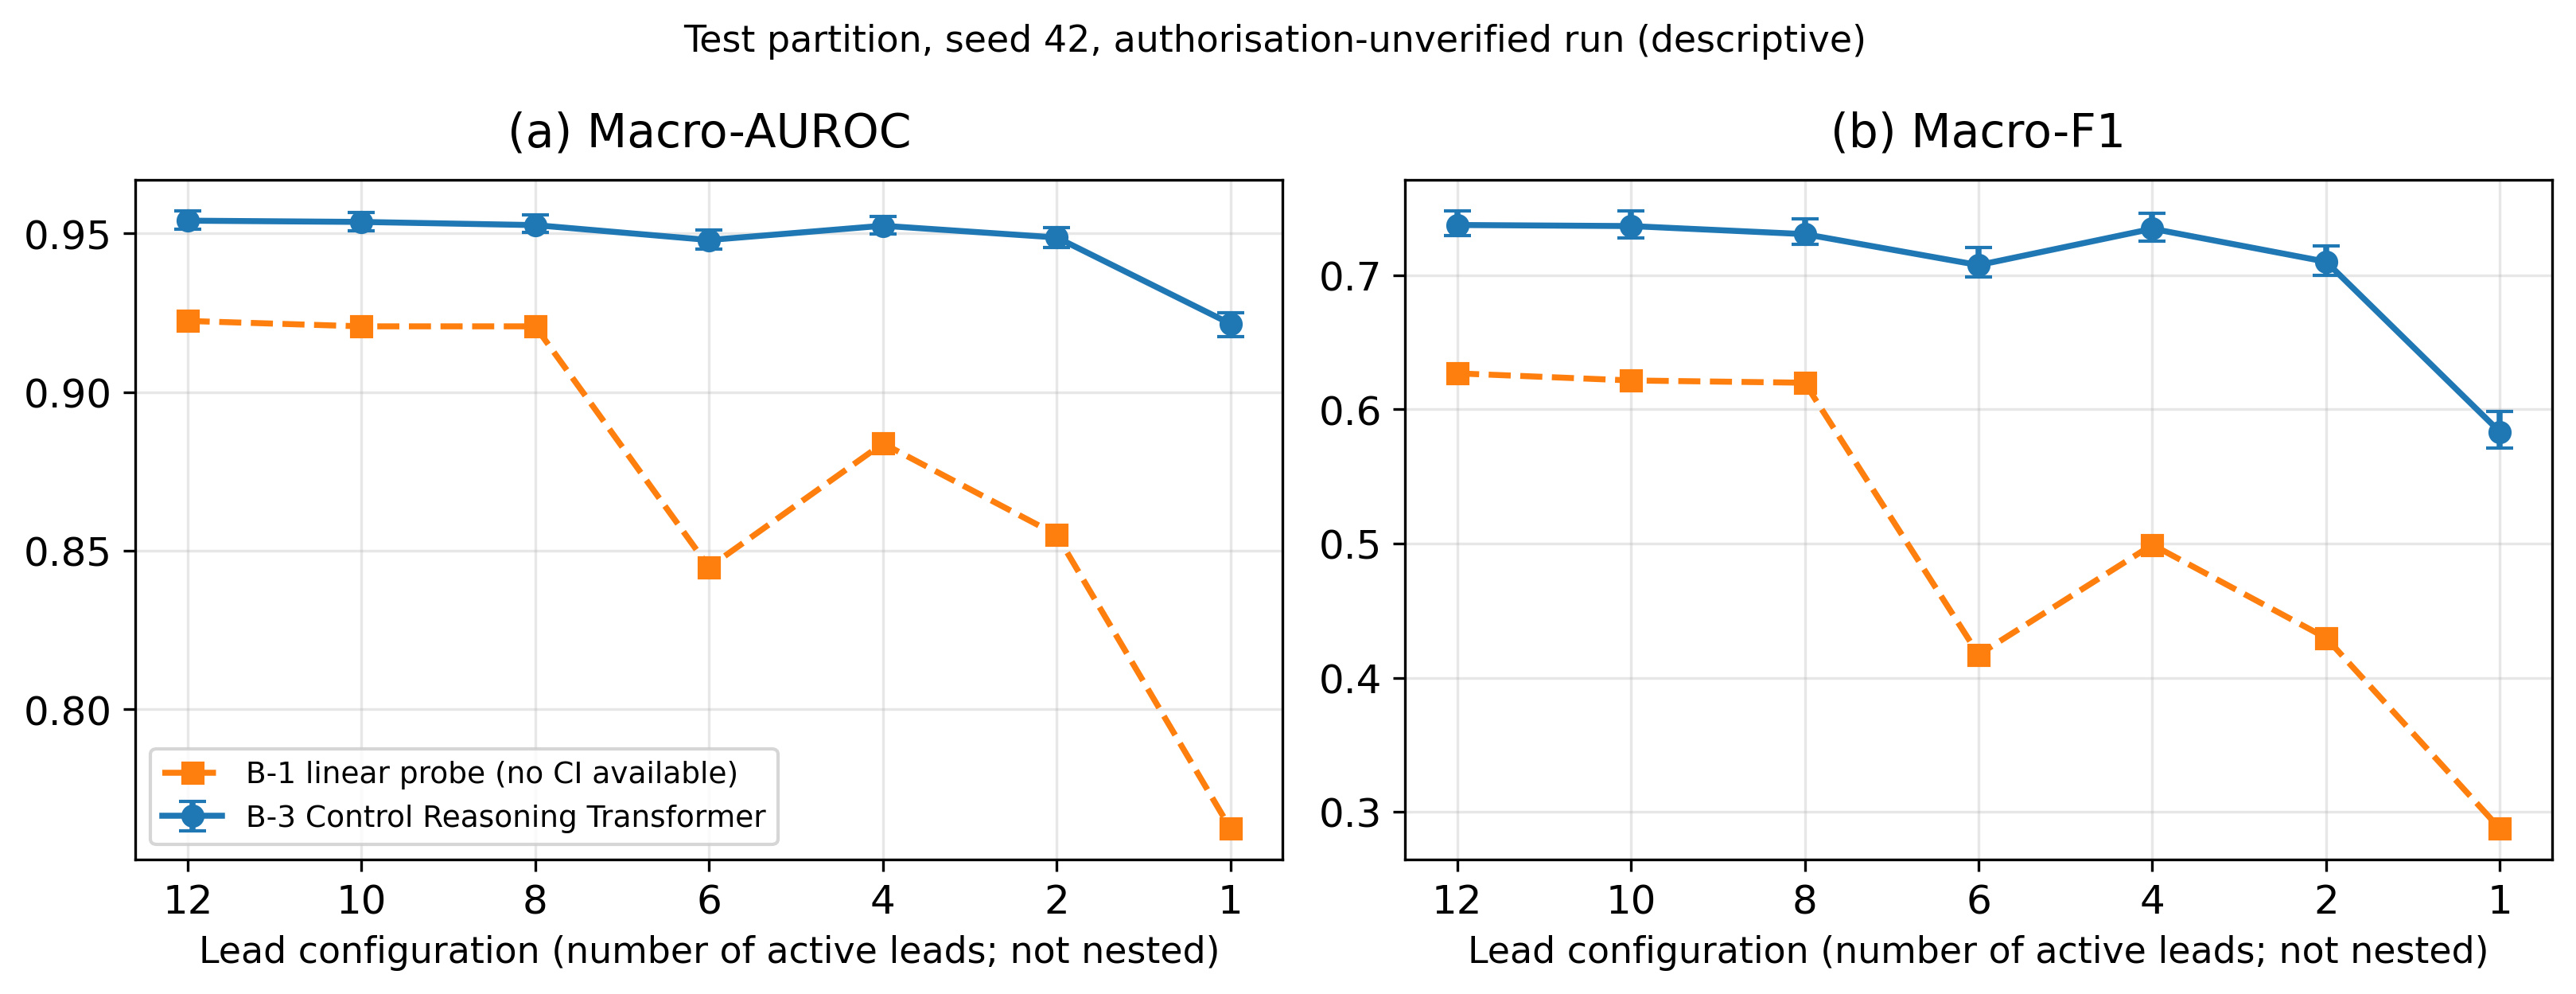
\includegraphics[width=\textwidth]{images/fig4_1_macro_metrics_by_configuration.jpg}
\caption{Test Macro-AUROC and Macro-F1 by Lead Configuration (B-3 with 95\% bootstrap intervals; B-1 point estimates only, since no intervals can be computed for it; drawn directly from the saved result files)}
\label{fig:ch4_1}
\end{figure}

Three features of the results stand out. First, removing the four derived limb leads changes almost nothing: from 12 to 10 to 8 leads, the macro-AUROC moves from 0.9540 to 0.9536 to 0.9526 and the macro-F1 from 0.7375 to 0.7367 to 0.7307, and the confidence intervals overlap. This is expected, because leads III, aVR, aVL and aVF are linear combinations of leads I and II (Section 3.3.5). The 10- and 8-lead configurations hide these leads from the model but remove no electrical information.

Second, performance does not fall steadily with the number of leads. The 4-lead configuration (macro-AUROC 0.9524, macro-F1 0.7347) is better than the 6-lead configuration (0.9479, 0.7076), and the 2-lead configuration (0.9487, 0.7101) is about as good as the 6-lead one. The configurations are not nested. The 6-lead configuration keeps all six limb leads but no chest lead, whereas the 4-lead and 2-lead configurations keep chest lead V1. The results therefore suggest that, for these eight conditions, V1 carries information that the full set of limb leads does not provide. This agrees with the observation that a well-chosen small lead subset can classify ECG abnormalities as well as larger sets \cite{LAI2021LEADSELECTION}. The lead-count ordering of the configurations is therefore not an ordering of information content. The difference between the 4- and 6-lead configurations (0.0045 in macro-AUROC and 0.0271 in macro-F1) is larger than the variation between seeds in either configuration on the validation partition (Table~\ref{tab:ch4_6}), and the macro-F1 intervals do not overlap, but no paired test of the difference is available.

Third, the single-lead configuration is clearly the weakest: its macro-AUROC is 0.9215 and its macro-F1 is 0.5832, against 0.9487 and 0.7101 for the 2-lead configuration. Section~\ref{sec:ch4_4_4} shows that this drop is concentrated in a few conditions.

The Diagnostic Failure Boundary of the protocol is defined from the ratio of each configuration's macro-F1 to the 12-lead macro-F1, with bootstrap intervals for that ratio. Those intervals are not implemented, so no Diagnostic Failure Boundary is reported, although the point estimates above show where macro-F1 falls most.

\subsection{Per-Condition Performance}\label{sec:ch4_4_4}

Table~\ref{tab:ch4_8} gives the per-condition F1 of the Control Reasoning Transformer on the test partition, and Figure~\ref{fig:ch4_2} shows the same values. The number of known labels and positives behind each condition is given in Table~\ref{tab:ch4_3}; these denominators are the same in every configuration.


\begin{table}[htbp]
\centering
\small
\setlength{\tabcolsep}{2pt}
\renewcommand{\arraystretch}{1.12}
\setstretch{1.0}
\caption[Test F1 per Condition]{Test F1 per Condition at Threshold 0.5 (Seed 42, Calibrated, Descriptive)}\label{tab:ch4_8}
\begin{tabular}{|c|c|c|c|c|c|c|c|}
\hline
\textbf{Condition} & \textbf{12} & \textbf{10} & \textbf{8} & \textbf{6} & \textbf{4} & \textbf{2} & \textbf{1} \\ \hline
NORM & 0.7778 & 0.7761 & 0.7732 & 0.7657 & 0.7701 & 0.7562 & 0.7310 \\ \hline
AFIB & 0.8028 & 0.7979 & 0.7966 & 0.7700 & 0.8036 & 0.7755 & 0.7479 \\ \hline
RBBB & 0.7855 & 0.7728 & 0.7363 & 0.6725 & 0.7785 & 0.7707 & 0.1266 \\ \hline
LBBB & 0.7910 & 0.7985 & 0.7955 & 0.7750 & 0.7821 & 0.7481 & 0.4565 \\ \hline
SBRAD & 0.8577 & 0.8599 & 0.8561 & 0.8593 & 0.8787 & 0.8539 & 0.8355 \\ \hline
STACH & 0.9121 & 0.9139 & 0.9165 & 0.9035 & 0.9121 & 0.9116 & 0.9058 \\ \hline
1AVB & 0.4230 & 0.4348 & 0.4315 & 0.4035 & 0.4410 & 0.3925 & 0.4172 \\ \hline
MI & 0.5500 & 0.5394 & 0.5395 & 0.5112 & 0.5116 & 0.4720 & 0.4451 \\ \hline
\end{tabular}
\end{table}

{\small Source: \path{runs/module4_v3/metrics/test_evaluation_summary.json}.}

\begin{figure}[htbp]
\centering
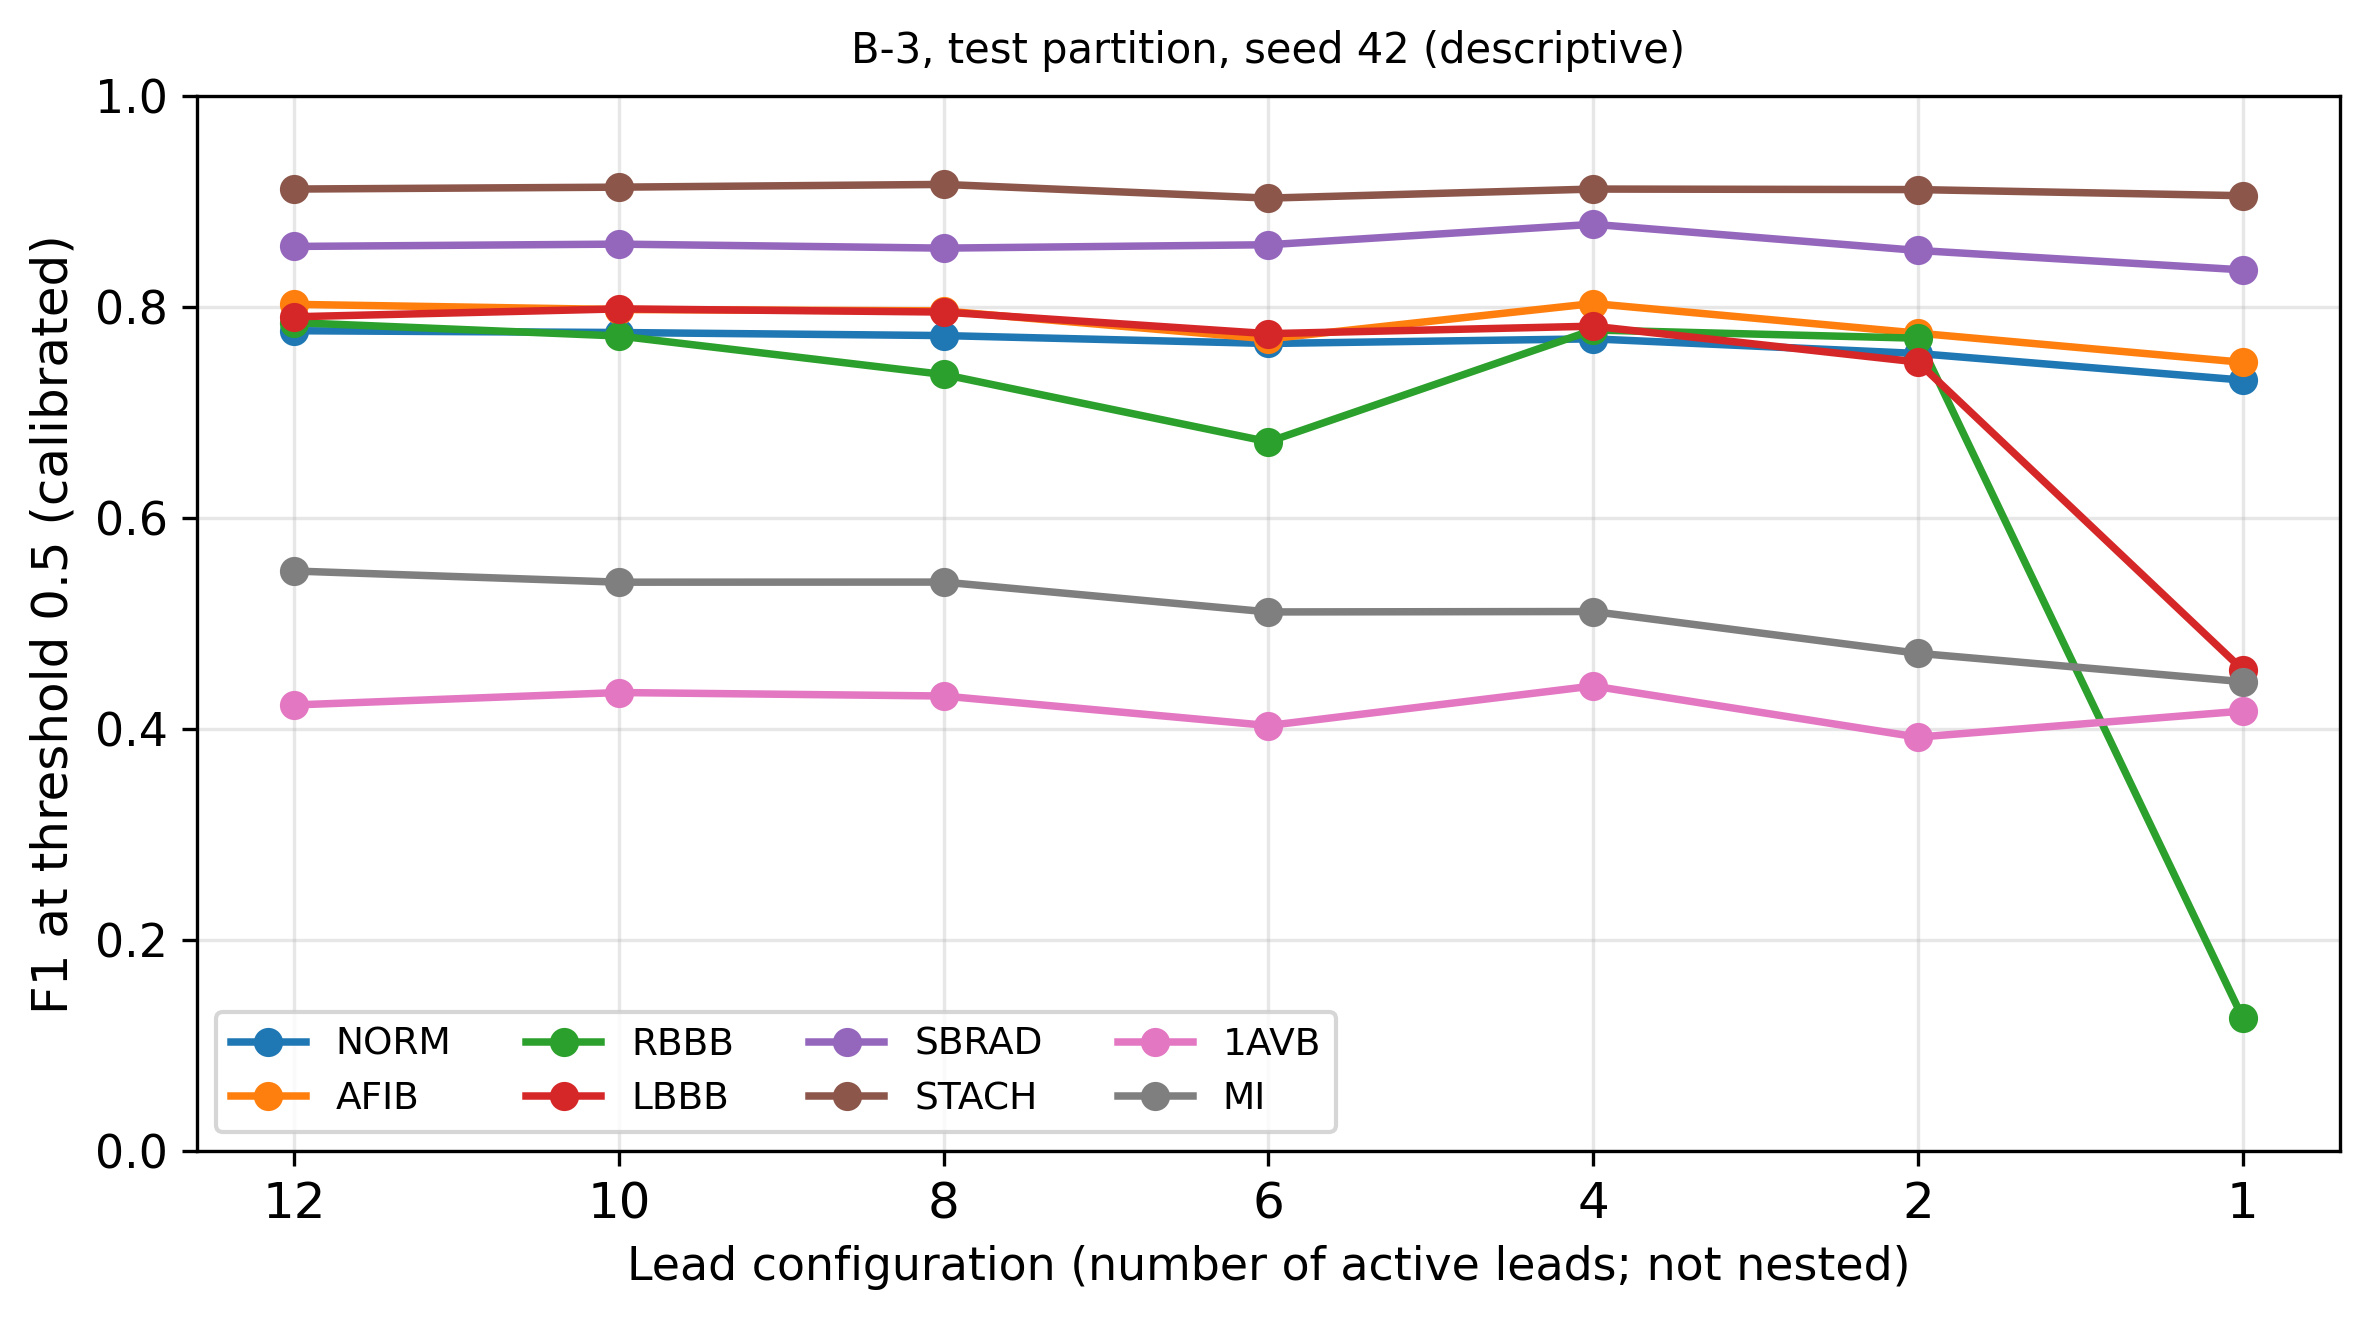
\includegraphics[width=\textwidth]{images/fig4_2_per_condition_f1.jpg}
\caption{Test F1 per Condition by Lead Configuration (B-3, seed 42; drawn directly from the saved test summary)}
\label{fig:ch4_2}
\end{figure}

The per-condition AUROC, from the same file, shows the same picture. Except for myocardial infarction, every condition kept an AUROC of at least 0.917 down to two leads; with lead II alone, the AUROC ranged from 0.8011 for myocardial infarction to 0.9940 for sinus tachycardia. The conditions fall into three groups.

\textbf{Rate-based conditions.} Sinus bradycardia and sinus tachycardia keep an AUROC of at least 0.982 and an F1 of at least 0.835 in every configuration, including the single-lead one. Both are defined mainly by heart rate, which can be measured from any lead that shows the QRS complexes. Lead II is retained in every configuration, so the heart rate measured from it, which reaches the model through the interval token, is the same in all seven (Section 3.3.7).

\textbf{Conduction blocks.} Right bundle branch block depends on chest lead V1 in a clear way. Its F1 is 0.7855 with all leads, falls to 0.6725 in the 6-lead configuration, which has no chest leads, recovers to 0.7785 and 0.7707 in the 4- and 2-lead configurations, which keep V1, and collapses to 0.1266 with lead II alone, where its recall is 0.074 and its AUROC 0.8408, against 0.9642 with all leads. Left bundle branch block degrades less: its F1 is between 0.748 and 0.799 down to two leads and falls to 0.4565 with one lead, where its AUROC is 0.9441. This pattern is consistent with the project schema, which assigns V1 and V6 to right bundle branch block (Table 3.2), but it does not show that the model uses those leads for the right reasons; establishing that is the purpose of the grounding gate.

\textbf{Low-F1 conditions.} First-degree atrioventricular block and myocardial infarction have the lowest F1 in every configuration. For first-degree atrioventricular block, the AUROC is high (0.9501 with all leads), but the F1 is only 0.4230, because the recall at threshold 0.5 is 0.32: only 149 test recordings receive a calibrated probability above 0.5 (92 true and 57 false positives), against 286 positive recordings. Myocardial infarction has the lowest AUROC (0.8475 with all leads, 0.8011 with one lead). Its criteria in the project schema depend on ST elevation or Q waves in contiguous leads of one territory (Table 3.2), Q waves are not among the extracted observations, and its labels come from three different labelling processes (Section~\ref{sec:ch4_1_1}).

\subsection{Performance by Cohort}\label{sec:ch4_4_5}

With all leads, the test macro-AUROC was 0.9476 for PTB-XL (4,358 recordings), 0.9509 for Chapman-Shaoxing (2,028) and 0.9379 for MIMIC-IV-ECG (989), and the corresponding macro-F1 values were 0.6767, 0.6775 and 0.7083. With lead II alone, the macro-AUROC was 0.9163, 0.9260 and 0.8981 (source: \texttt{dataset\_breakdown} field of the test summary).

The model performs at a similar level on all three cohorts, and the configuration pattern of Section~\ref{sec:ch4_4_3}, including the advantage of the 4-lead over the 6-lead configuration, appears in each of them (4-lead and 6-lead macro-AUROC: 0.9431 and 0.9406 for PTB-XL, 0.9618 and 0.9488 for Chapman-Shaoxing, 0.9367 and 0.9318 for MIMIC-IV-ECG). The macro-F1 of each cohort is lower than the macro-F1 of the pooled test partition. A likely reason is that some conditions have few positives in a single cohort, which lowers the cohort's per-condition F1; the project's post-evaluation audit records, for example, only 8 positive myocardial infarction recordings among the Chapman-Shaoxing test recordings. The MIMIC-IV-ECG results measure agreement with machine-generated statements rather than with clinicians, so they are not directly comparable with the other two cohorts \cite{REYNA2022ISSUES}. Because the three cohorts were pooled and split together, none of these results is an external validation on an unseen cohort. Nor are they comparable with published PTB-XL benchmarks \cite{STRODTHOFF2021PTBXL}, which use PTB-XL's own folds and label sets.

\subsection{Comparison Models}\label{sec:ch4_4_6}

The comparison models were evaluated on the same 7,375 test recordings and configurations (experiment E9). Table~\ref{tab:ch4_9} compares the linear probe (B-1) with the Control Reasoning Transformer (B-3).

{
\setlength{\tabcolsep}{2pt}
\renewcommand{\arraystretch}{1.12}
\begin{table}[htbp]
\centering
\footnotesize
\setstretch{1.0}
\caption[Linear Probe versus Control Reasoning Transformer]{Test Performance of the Linear Probe (B-1) and the Control Reasoning Transformer (B-3) (Descriptive)}\label{tab:ch4_9}
\begin{tabular}{|c|c|c|c|c|}
\hline
\textbf{Configuration} & \textbf{B-1 macro-AUROC} & \textbf{B-3 macro-AUROC} & \textbf{B-1 macro-F1} & \textbf{B-3 macro-F1} \\ \hline
12-lead & 0.9224 & 0.9540 & 0.6269 & 0.7375 \\ \hline
10-lead & 0.9207 & 0.9536 & 0.6216 & 0.7367 \\ \hline
8-lead & 0.9207 & 0.9526 & 0.6199 & 0.7307 \\ \hline
6-lead & 0.8448 & 0.9479 & 0.4172 & 0.7076 \\ \hline
4-lead & 0.8838 & 0.9524 & 0.4991 & 0.7347 \\ \hline
2-lead & 0.8550 & 0.9487 & 0.4296 & 0.7101 \\ \hline
1-lead & 0.7624 & 0.9215 & 0.2874 & 0.5832 \\ \hline
\end{tabular}
\end{table}
}

{\small Source: \path{runs/module4_v3/metrics/comprehensive_baseline_comparison.json}.}

The linear probe is a logistic regression for each condition, fitted on the frozen 12-lead representations of the training partition and applied without calibration at a threshold of 0.5. With all leads, it reaches a macro-AUROC of 0.9224, which shows that the frozen foundation-model representation already separates the eight conditions well. The Control Reasoning Transformer is higher in every configuration, by 0.03 in macro-AUROC and 0.11 in macro-F1 with 12, 10 or 8 leads, and by 0.24 to 0.30 in macro-F1 in the 6-, 4-, 2- and 1-lead configurations. The linear probe follows broadly the same pattern across configurations as the representation drift of Section~\ref{sec:ch4_4_7}: it is almost unchanged at 10 and 8 leads, falls most at 6 and 1 leads, and is better at 4 leads than at 6.

This comparison is descriptive. The two models differ at once in capacity, in training (the probe saw only 12-lead representations), in their observation and lead-availability inputs and in calibration, so the gap cannot be attributed to any one factor without ablations, which have not been run. The probe's per-recording predictions were not saved, so no paired intervals are available (Section~\ref{sec:ch4_3_2}).

The class-prevalence model (B-0) has a macro-AUROC of 0.5 and a macro-F1 of 0 by construction. The rule-engine model (B-2) is withdrawn as a comparison: it never predicts bundle branch block, because the extracted QRS duration never reaches 120 ms (Section~\ref{sec:ch4_4_8}), and the main branch of its atrial fibrillation rule never matches the extractor's label "Atrial Fibrillation / Irregular rhythm".

\subsection{Representation Stability}\label{sec:ch4_4_7}

Table~\ref{tab:ch4_10} gives the mean cosine similarity between the representation of each recording in a reduced configuration and its 12-lead representation, produced by the frozen foundation model (experiment E10).

\begin{table}[htbp]
\centering
\small
\setlength{\tabcolsep}{2pt}
\renewcommand{\arraystretch}{1.12}
\setstretch{1.0}
\caption{Mean Cosine Similarity to the 12-Lead Representation}\label{tab:ch4_10}
\begin{tabular}{|>{\raggedright\arraybackslash}p{0.15\textwidth}|>{\raggedright\arraybackslash}p{0.28\textwidth}|>{\raggedright\arraybackslash}p{0.23\textwidth}|>{\raggedright\arraybackslash}p{0.25\textwidth}|}
\hline
\textbf{Configuration} & \textbf{All partitions (36,888 recordings)} & \textbf{Test partition (7,375 recordings)} & \textbf{Standard deviation (all partitions)} \\ \hline
10-lead & 0.9981 & 0.9980 & 0.0021 \\ \hline
8-lead & 0.9971 & 0.9971 & 0.0027 \\ \hline
6-lead & 0.8775 & 0.8780 & 0.0621 \\ \hline
4-lead & 0.9041 & 0.9041 & 0.0520 \\ \hline
2-lead & 0.8762 & 0.8752 & 0.0621 \\ \hline
1-lead & 0.8144 & 0.8130 & 0.0849 \\ \hline
\end{tabular}
\par
{\small Source: \path{runs/module3_v1/reports/module3_cosine_similarity_summary.csv}.}
\end{table}

The representation changes very little when only derived leads are removed (similarity above 0.997) and changes most with a single lead (0.8144). Its ordering follows the classification results closely: the 4-lead representation stays closer to the 12-lead one than the 6-lead or 2-lead representations do, as the 4-lead classification results are better. The values measure the geometry of the representation, not diagnostic accuracy, and a lower similarity does not by itself mean lower accuracy, since the Control Reasoning Transformer was trained on the reduced representations as well.

Two cautions apply. Zero-masking changes the input distribution as well as the information available, and the two effects are hard to separate \cite{HOOKER2019ROAR}. In addition, ECG-FM is used outside its pretraining conditions (Section 3.3.6) \cite{MCKEEN2025ECGFM}, and record-level overlap between its pretraining data and the project's test recordings has not been checked.

\subsection{Clinical Observation Extractor}\label{sec:ch4_4_8}

The observation extractor was validated in a study of 250 MIMIC-IV-ECG recordings, sampled with seed 42 and compared with the measurements and statements produced by the dataset's automated interpretation program (\url{scripts/audit_clinical_observations.py}). The study was run on 6 October 2026, before the Module 4 freeze record was written on 15 October. The extractor source file was last modified on 23 September 2026, before the study, and its current SHA-256 hash matches the hash in the freeze record. The study therefore used the extractor code that was later frozen. The study did not record a code hash of its own.

Against the reference values, heart rate had a mean absolute error of 3.70 bpm (median 0.96 bpm; Pearson r = 0.866), the PR interval 21.57 ms (median 14.0 ms; r = 0.581) and the QRS duration 28.92 ms (median 26.0 ms; r = 0.255). Rhythm detection reached an F1 of 0.917 for sinus bradycardia, 0.681 for sinus tachycardia (sensitivity 0.517) and 0.475 for atrial fibrillation (sensitivity 0.633, precision 0.380, from 19 true and 31 false positives). The ST-segment and T-wave rules were not validated. The study labels the heart-rate measurement ``clinically validated'', although it compared it only with machine measurements (source: \texttt{reports/clinical\_observation\_validation.json}).



Heart rate, measured with the Pan–Tompkins-style detector of Section 3.3.7 \cite{PAN1985QRS}, agrees well with the machine measurements. The PR interval agrees only moderately, and the QRS duration agrees poorly. The reference values are themselves produced by an automated program, so the study measures agreement between two algorithms, not accuracy against a clinician; it is evidence of reasonableness rather than clinical validation.

The extracted observations of the training partition show two limitations directly. The extracted QRS duration of the 25,715 training recordings with a measurement lies between 50 and 110 ms, and none reaches 120 ms, because the QRS search window of ±60 ms at 100 Hz cannot measure a wider complex (Section 3.3.7). The PR interval lies between 100 and 250 ms, and 2,460 recordings exceed 200 ms. The rhythm labels written by the extractor are "Sinus rhythm" (13,673 recordings), "Sinus Bradycardia" (5,875), "Atrial Fibrillation / Irregular rhythm" (3,828), "Sinus Tachycardia" (2,239) and "Indeterminate rhythm" (210). Only "Sinus rhythm" matches the rhythm vocabulary of the context builder, so the other 12,152 training recordings (47.1\%) receive the same out-of-vocabulary rhythm token (Section 3.2).

The Control Reasoning Transformer therefore receives capped QRS values and a merged rhythm token, so the observation tokens cannot be assumed to contribute the information they were designed to provide. The same limits will matter more for the grounding gate: with the current extractor, a bundle branch block claim could never be supported by a measured QRS duration (Section 3.3.9).

\subsection{Discussion}\label{sec:ch4_4_9}

The first-half experiments establish a complete, reproducible classification pipeline across seven lead configurations and three cohorts. The frozen foundation model gives a representation that separates the eight conditions well (linear-probe macro-AUROC 0.9224 with all leads), and the Control Reasoning Transformer, trained once over all configurations, reaches a test macro-AUROC of 0.9540 with all leads and keeps it above 0.947 down to two leads. Diagnostic performance falls clearly only with a single lead, and it falls unevenly across conditions: rate-based conditions are unaffected, while right bundle branch block depends visibly on the presence of V1.

These findings answer only the diagnostic half of the research question. A model can keep a high AUROC on a single lead by relying on features that a cardiologist would not accept as evidence, and attention-based traces cannot settle this \cite{JAIN2019ATTENTION}; measuring it requires the grounding gate.

Several factors other than the reasoning model could explain parts of the results: the cohorts' different labelling processes, the encoder's non-native inputs and possible pretraining overlap, zero-masking, the observation extractor's limitations and the duplicated recordings. None of them invalidates the results as descriptive measurements, but together they limit how far the results can be generalised.

The test results are a single seed of a single authorisation-unverified run, and they should be confirmed by an authorised, separately versioned evaluation before any confirmatory claim is made. Section 4.3.1 lists the parts of the research programme for which no results exist yet.